% =============================================================================
% Two-Stage Grokking and Backward BFS in a Small Transformer
% Research Writeup — Phase 4
% =============================================================================

\documentclass[11pt, a4paper]{article}

\usepackage{amsmath, amssymb, amsthm}
\usepackage{geometry}
\usepackage[colorlinks=true, linkcolor=blue, urlcolor=blue, citecolor=blue]{hyperref}
\usepackage{booktabs}
\usepackage{array}
\usepackage{xcolor}
\usepackage{float}
\usepackage{parskip}
\usepackage{titlesec}
\usepackage{enumitem}
\usepackage{microtype}
\usepackage{graphicx}
\usepackage{caption}
\usepackage{subcaption}
\usepackage{natbib}
\usepackage{pgfplots}
\pgfplotsset{compat=1.18}

\geometry{margin=2.5cm}

% Math macros
\DeclareMathOperator{\softmax}{softmax}
\DeclareMathOperator{\LN}{LN}
\newcommand{\INF}{\textsc{inf}}
\newcommand{\PAD}{\textsc{pad}}
\newcommand{\EDGE}{\textsc{edge}}
\newcommand{\QRY}{\textsc{qry}}
\newcommand{\pp}{\,pp}  % percentage points

\titlespacing*{\section}{0pt}{1.8em}{0.8em}
\titlespacing*{\subsection}{0pt}{1.2em}{0.5em}

% -----------------------------------------------------------------------
\title{%
  \textbf{Two-Stage Grokking and Backward BFS\\
          in a Small Transformer on a Graph-Distance Task}
}
\author{Shukanth Jojodae}
\date{May 19, 2026}
% -----------------------------------------------------------------------

\begin{document}
\maketitle
\tableofcontents
\newpage

% =============================================================================
\begin{abstract}
% =============================================================================

A transformer can reach the same validation accuracy through two
mechanistically distinct algorithms: first by learning a statistical
shortcut, then by discarding it and replacing it with genuine structural
reasoning.  We demonstrate this in a two-layer attention-only
transformer trained on directed graph shortest-path queries.  Training
exhibits a double-grokking pattern --- grokking being a phenomenon
where generalization emerges long after memorization --- with two
successive sharp improvements in validation accuracy separated by a
plateau.  The first transition corresponds to the construction of a
PAD-token logit bias: the model exploits the fixed structure of padding
positions to inject a constant prediction offset, achieving above-chance
accuracy without performing any graph computation.  The second
transition dismantles this shortcut and installs a genuine
graph-structural circuit: Layer~0 implements a token-identity attention
pattern that collects the immediate neighborhood of the destination
node, and Layer~1 checks whether the source can reach any of those
neighbors in one hop --- a partial two-step backward breadth-first
search.  This mechanism handles distance-1 and distance-2 queries well
(99.4\% and 87.0\% validation accuracy) but fails systematically on
distance-3 (23.8\%), an architectural limitation of the two-layer
design.  We trace this account using weight-norm analysis, OV and QK
circuit decomposition, causal ablation, and the logit lens, and
identify the positional component of Layer~0's value vectors as the
primary open question for a complete mechanistic account.

\end{abstract}

% =============================================================================
\section{Introduction}
\label{sec:intro}
% =============================================================================

Grokking --- a phenomenon in which a neural network generalizes to
held-out data long after it has memorized the training set --- was
identified by \citet{power2022grokking} in small transformers trained
on algorithmic tasks.  A network first saturates training accuracy
(memorization), then continues training for thousands of additional
steps before validation accuracy suddenly jumps: a delayed phase
transition in generalization.  The original work studied modular
arithmetic and group composition; the mechanism underlying the
transition remained largely opaque.

Grokking creates an unusual opportunity for mechanistic interpretability.
During the long plateau between memorization and generalization, the
model's parameters are changing continuously while validation accuracy
is not.  Something is reorganizing internally.  If we can read the
model's internal representations at multiple checkpoints during
training, we can catch that reorganization in the act: what computation
did the model build, and what did it discard?

We study this in a setting designed to make the internal algorithm
recoverable.  A two-layer attention-only transformer is trained to
predict shortest-path lengths between pairs of nodes in small directed
graphs.  Directed graphs are chosen deliberately: asymmetric
reachability --- the path from $A$ to $B$ may not equal the path from
$B$ to $A$ --- blocks the symmetry-based shortcuts available in
undirected graphs and forces the model to develop richer internal
representations.  The task has a known algorithmic solution
(breadth-first search, BFS), a finite answer space (distances 1, 2, 3,
or unreachable), and enough structure to make circuit-level analysis
tractable.  The model is kept small --- two layers, two heads per
layer, approximately 140{,}000 parameters --- so that every component
can be examined directly.

\paragraph{What we find.}
The central question is: does the model learn BFS?  The answer is yes,
partially.  The fully trained model implements a two-step backward BFS
from the destination node.  Layer~0 contains an attention head (L0H1)
whose query-key circuit matches destination-node tokens to edge
positions in the sequence, collecting the immediate neighborhood of the
destination.  Layer~1 reads this neighborhood information and checks
whether the source node can reach any of those neighbors in a single
hop.  This two-step computation handles paths of length 1 and 2 well
(99.4\% and 87.0\%) but fails on paths of length 3 (23.8\%), which
would require a third BFS step the architecture cannot perform.

Training reaches this algorithm through two grokking events, not one.
The first transition produces a model that exploits a statistical
shortcut --- attending to padding positions and injecting a constant
logit bias --- without performing any graph computation.  The second
transition dismantles this shortcut and replaces it with the genuine
BFS circuit.  The mechanistic distinction between the two stages is the
paper's central contribution.

\paragraph{Related work.}
The closest prior work is \citet{cohen2025spectral}, who study
shortest-path interpretability in transformers trained on \emph{undirected}
graphs, analyzing the fully converged model.  Our setting differs in three
ways that matter mechanistically.  First, we use directed graphs, where
asymmetric reachability prevents the symmetry-based shortcuts that
undirected settings allow, forcing the model to develop a richer internal
representation.  Second, we study the full training trajectory rather than
only the final model, which reveals the intermediate shortcut phase that
a converged-only analysis would miss entirely.  Third, the two-stage
grokking dynamic --- shortcut construction followed by shortcut
replacement --- is a finding about the \emph{process} of generalization,
not just its end state, and has no analogue in prior interpretability
work on algorithmic tasks.

\paragraph{Paper structure.}
Section~\ref{sec:task} defines the task, tokenization scheme, and
model architecture.  Section~\ref{sec:training} describes training
dynamics and establishes the two-stage grokking observation.
Section~\ref{sec:circuits} traces the circuits responsible for each
stage using weight-norm analysis, OV/QK decomposition, and causal
ablation.  Section~\ref{sec:algorithm} characterizes the learned
algorithm using the logit lens.  Section~\ref{sec:discussion} discusses
implications and future directions.

% =============================================================================
\section{Task, Tokenization, and Model}
\label{sec:task}
% =============================================================================

\subsection{Task definition}

Let $G = (V, E)$ be a directed unweighted graph with $|V| = n$ nodes
labelled $0, \ldots, n{-}1$ and $E \subseteq V \times V$ with no
self-loops.  Given source $s \in V$ and destination $d \in V$ with
$s \neq d$, the model must predict
\[
  y = \begin{cases}
    \mathrm{dist}(s, d) & \text{if } d \text{ is reachable from } s, \\
    \INF                & \text{otherwise,}
  \end{cases}
\]
where $\mathrm{dist}(s, d)$ is the number of edges in the shortest
directed path from $s$ to $d$.

All experiments use $n = 4$ nodes.  Graphs are sampled with random
directed edges, density $\approx 0.4$, using NetworkX's BFS for
ground-truth labels.  The answer space is $\{1, 2, 3, \INF\}$; a path
of length~0 is excluded since $s \neq d$ is enforced.

\subsection{Tokenization}

The graph and query are encoded as a fixed-length integer sequence:
\[
  \underbrace{[\EDGE, u_1, v_1]}_{\text{edge 1}}\;
  \underbrace{[\EDGE, u_2, v_2]}_{\text{edge 2}}\;
  \cdots\;
  \underbrace{[\PAD, \PAD, \PAD]}_{\text{unused slots}}\;
  \cdots\;
  \underbrace{[\QRY, s, d]}_{\text{query}}
\]

Each directed edge $u \to v$ is represented as a three-token triplet
$[\EDGE, u, v]$.  Up to $E_{\max} = 6$ edge triplets are packed
before the query; unused positions are filled with \PAD\ triplets.
The query occupies the final three positions, so sequence length is
$L = 3 \times 6 + 3 = 21$ tokens.

Edge order is shuffled randomly for each training example.  This
prevents the model from exploiting positional shortcuts (e.g., ``the
useful edge is always at position 3'') and forces it to learn an
order-invariant algorithm.

\paragraph{Vocabulary.}
For $n = 4$, the vocabulary has 8 tokens: node identifiers 0--3,
\EDGE, \QRY, \PAD, and \INF.  Node tokens double as distance labels:
token~1 encodes both the node~1 identifier and the answer
``distance 1.''  \INF\ is an output-only token; it never appears in
input sequences.  Logits are computed over all 8 vocabulary entries;
tokens that can never be a correct answer (node~0, \EDGE, \QRY, \PAD)
are called \emph{impossible-answer tokens}.

\paragraph{Prediction position.}
The model reads out logits from the last token position --- the \texttt{dst}
position within the \QRY\ triplet.  This is a natural choice: the
destination node is the only position with direct access to the query
and is the last position in the sequence, giving it access to all
upstream context via attention.

\paragraph{Train/validation split.}
The split is by graph structure, not by query.  All 12 directed pairs
$(s, d)$ from a given graph are assigned together to either training or
validation.  The model is never evaluated on a graph it has seen during
training, only on unseen topologies.  The dataset contains 200 graphs:
160 training graphs (1{,}920 samples) and 40 validation graphs (480
samples).

\subsection{Model architecture}

The model is a two-layer, attention-only transformer with no MLP
blocks.  Attention-only models are the preferred architecture for
mechanistic interpretability: without MLP layers, every computation is
an attention head, and each head's contribution is fully described by
its OV and QK circuits (Section~\ref{sec:circuits}).

\begin{table}[H]
\centering
\begin{tabular}{@{}ll@{}}
\toprule
Hyperparameter & Value \\
\midrule
Layers             & 2 \\
Heads per layer    & 2 \\
Residual dimension $d_{\mathrm{model}}$ & 128 \\
Head dimension $d_{\mathrm{head}}$      & 64 \\
Vocabulary size    & 8 \\
Sequence length    & 21 \\
Total parameters   & $\approx$140{,}000 \\
\bottomrule
\end{tabular}
\caption{Model configuration for all experiments.}
\label{tab:model}
\end{table}

The forward pass is:
\begin{align}
  x^{(0)} &= W_E[\mathrm{tokens}] + W_{\mathrm{pos}}, \\
  x^{(l)} &= x^{(l-1)} + \mathrm{MHA}_l\!\left(\LN_l(x^{(l-1)})\right),
  \quad l = 1, 2, \\
  \mathrm{logits} &= W_U\, \LN_{\mathrm{final}}\!\left(x^{(2)}_{-1}\right),
\end{align}
where $W_E \in \mathbb{R}^{8 \times 128}$ is the token embedding
matrix, $W_{\mathrm{pos}} \in \mathbb{R}^{21 \times 128}$ is a
learned positional embedding, and $W_U \in \mathbb{R}^{128 \times 8}$
is the unembedding matrix.  Pre-norm LayerNorm is applied before each
attention block.  No biases are used in the attention projections, which
keeps the OV and QK circuit decompositions exact (no additive offset
terms to track).

\paragraph{Training.}
The model is trained with AdamW, learning rate $10^{-3}$, weight decay
$\lambda = 0.4$, batch size 128, for 200{,}000 gradient steps.
Checkpoints are saved every 2{,}000 steps, producing 100 checkpoints
that form the experimental substrate for all interpretability analyses.

% =============================================================================
\section{Training Dynamics: Two-Stage Grokking}
\label{sec:training}
% =============================================================================

\subsection{The grokking phenomenon}

Grokking arises from a competition between two forces operating on
opposite timescales.  Gradient descent rapidly finds a high-norm
memorized solution that fits all training examples.  Weight decay
continuously shrinks every parameter, building slow pressure toward a
lower-norm solution.  After enough steps, weight decay overcomes
memorization and the model reorganizes into a compact solution that
generalizes --- validation accuracy jumps sharply.

The weight decay value $\lambda = 0.4$ is chosen to be strong enough
to eventually force this reorganization while still allowing full
memorization to occur first.  In preliminary experiments at
$\lambda = 0.2$, we observed a single sharp transition rather than two
stages, suggesting the timescale separation may depend on weight decay
strength.  At $\lambda = 0.4$, the transition splits into two distinct
events.

\subsection{Two grokking transitions}

\begin{figure}[H]
\centering
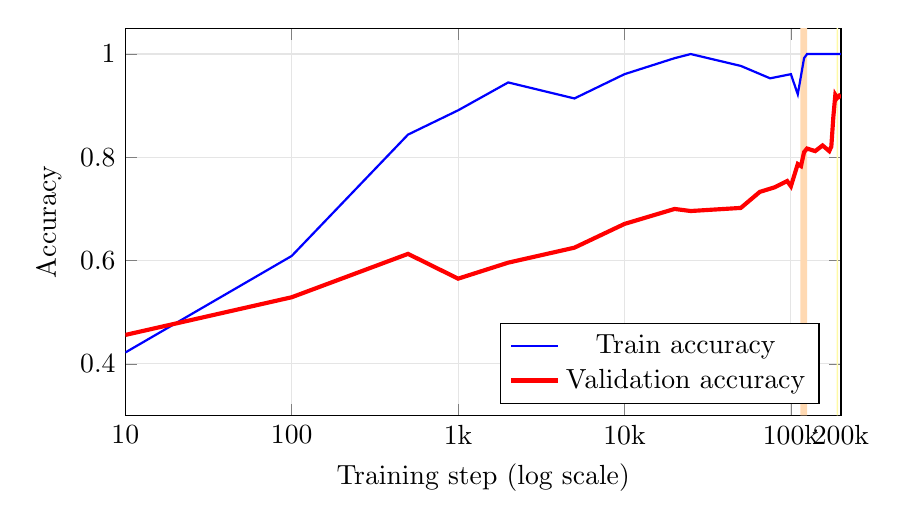
\begin{tikzpicture}
\begin{semilogxaxis}[
  width=0.88\textwidth, height=6.5cm,
  xlabel={Training step (log scale)}, ylabel={Accuracy},
  xmin=10, xmax=200000, ymin=0.3, ymax=1.05,
  xtick={10,100,1000,10000,100000,200000},
  xticklabels={10,100,1k,10k,100k,200k},
  legend pos=south east, grid=major, grid style={gray!20},
]
\addplot[fill=orange!30, draw=none, forget plot]
  coordinates {(114000,0.3)(114000,1.05)(125000,1.05)(125000,0.3)} \closedcycle;
\addplot[fill=yellow!35, draw=none, forget plot]
  coordinates {(188000,0.3)(188000,1.05)(192000,1.05)(192000,0.3)} \closedcycle;
\addplot[blue, thick] coordinates {
  (10,0.422)(100,0.609)(500,0.844)(1000,0.891)
  (2000,0.945)(5000,0.914)(10000,0.961)(20000,0.992)(25000,1.000)
  (50000,0.977)(75000,0.953)(100000,0.961)(110000,0.922)(120000,0.992)
  (125000,1.000)(140000,1.000)(160000,1.000)(175000,1.000)
  (180000,1.000)(190000,1.000)(200000,1.000)
};
\addplot[red, thick, line width=1.5pt] coordinates {
  (10,0.456)(100,0.529)(500,0.613)(1000,0.565)
  (2000,0.596)(5000,0.625)(10000,0.671)(20000,0.700)(25000,0.696)
  (50000,0.702)(65000,0.733)(80000,0.742)(95000,0.754)(100000,0.744)
  (110000,0.787)(115000,0.783)(120000,0.810)(125000,0.817)
  (140000,0.812)(155000,0.823)(170000,0.812)(175000,0.821)
  (180000,0.879)(185000,0.921)(190000,0.915)(195000,0.919)(200000,0.915)
};
\legend{Train accuracy, Validation accuracy}
\end{semilogxaxis}
\end{tikzpicture}
\caption{Training dynamics over 200{,}000 steps
  (\texttt{n\_nodes=4}, \texttt{n\_graphs=200}, $\lambda=0.4$).  The
  log x-axis reveals early memorization and two-stage generalization.
  Orange band: Stage~1 transition (steps 114k--125k), validation
  accuracy rises from $\sim$72\% to $\sim$82\%.  Yellow band: Stage~2
  transition (steps 188k--192k), validation accuracy rises from
  $\sim$82\% to $\sim$92\%.}
\label{fig:training-curve}
\end{figure}

Training proceeds through five qualitatively distinct phases:

\begin{enumerate}[noitemsep]
  \item \textbf{Memorization (steps 0--4k).}  Train accuracy reaches
    $\sim$95--100\%; validation accuracy rises only to $\sim$64\%.
    The model learns a high-norm lookup table.

  \item \textbf{Slow drift (steps 4k--105k).}  Validation accuracy
    rises slowly from 64\% to $\sim$75\% over 100{,}000 steps.  Weight
    decay is compressing the memorized solution but has not yet forced
    a transition.

  \item \textbf{Stage~1 transition (steps 114k--125k).}  Validation
    accuracy rises from $\sim$75\% to $\sim$82\%.  A partial
    generalizing circuit has formed.

  \item \textbf{Plateau II (steps 125k--188k).}  Validation accuracy
    oscillates between 79\% and 83\% for 63{,}000 steps.  The partial
    circuit is stable but something is still missing.

  \item \textbf{Stage~2 transition (steps 188k--192k).}  Validation
    accuracy jumps from $\sim$82\% to $\sim$92\%, where it stabilizes.
\end{enumerate}

The two transitions are not two instances of the same event.
Section~\ref{sec:circuits} shows they are mechanistically distinct:
Stage~1 builds a statistical shortcut; Stage~2 replaces it with
genuine structural computation.

\subsection{Weight-norm trajectories confirm two transitions}

\begin{figure}[H]
\centering
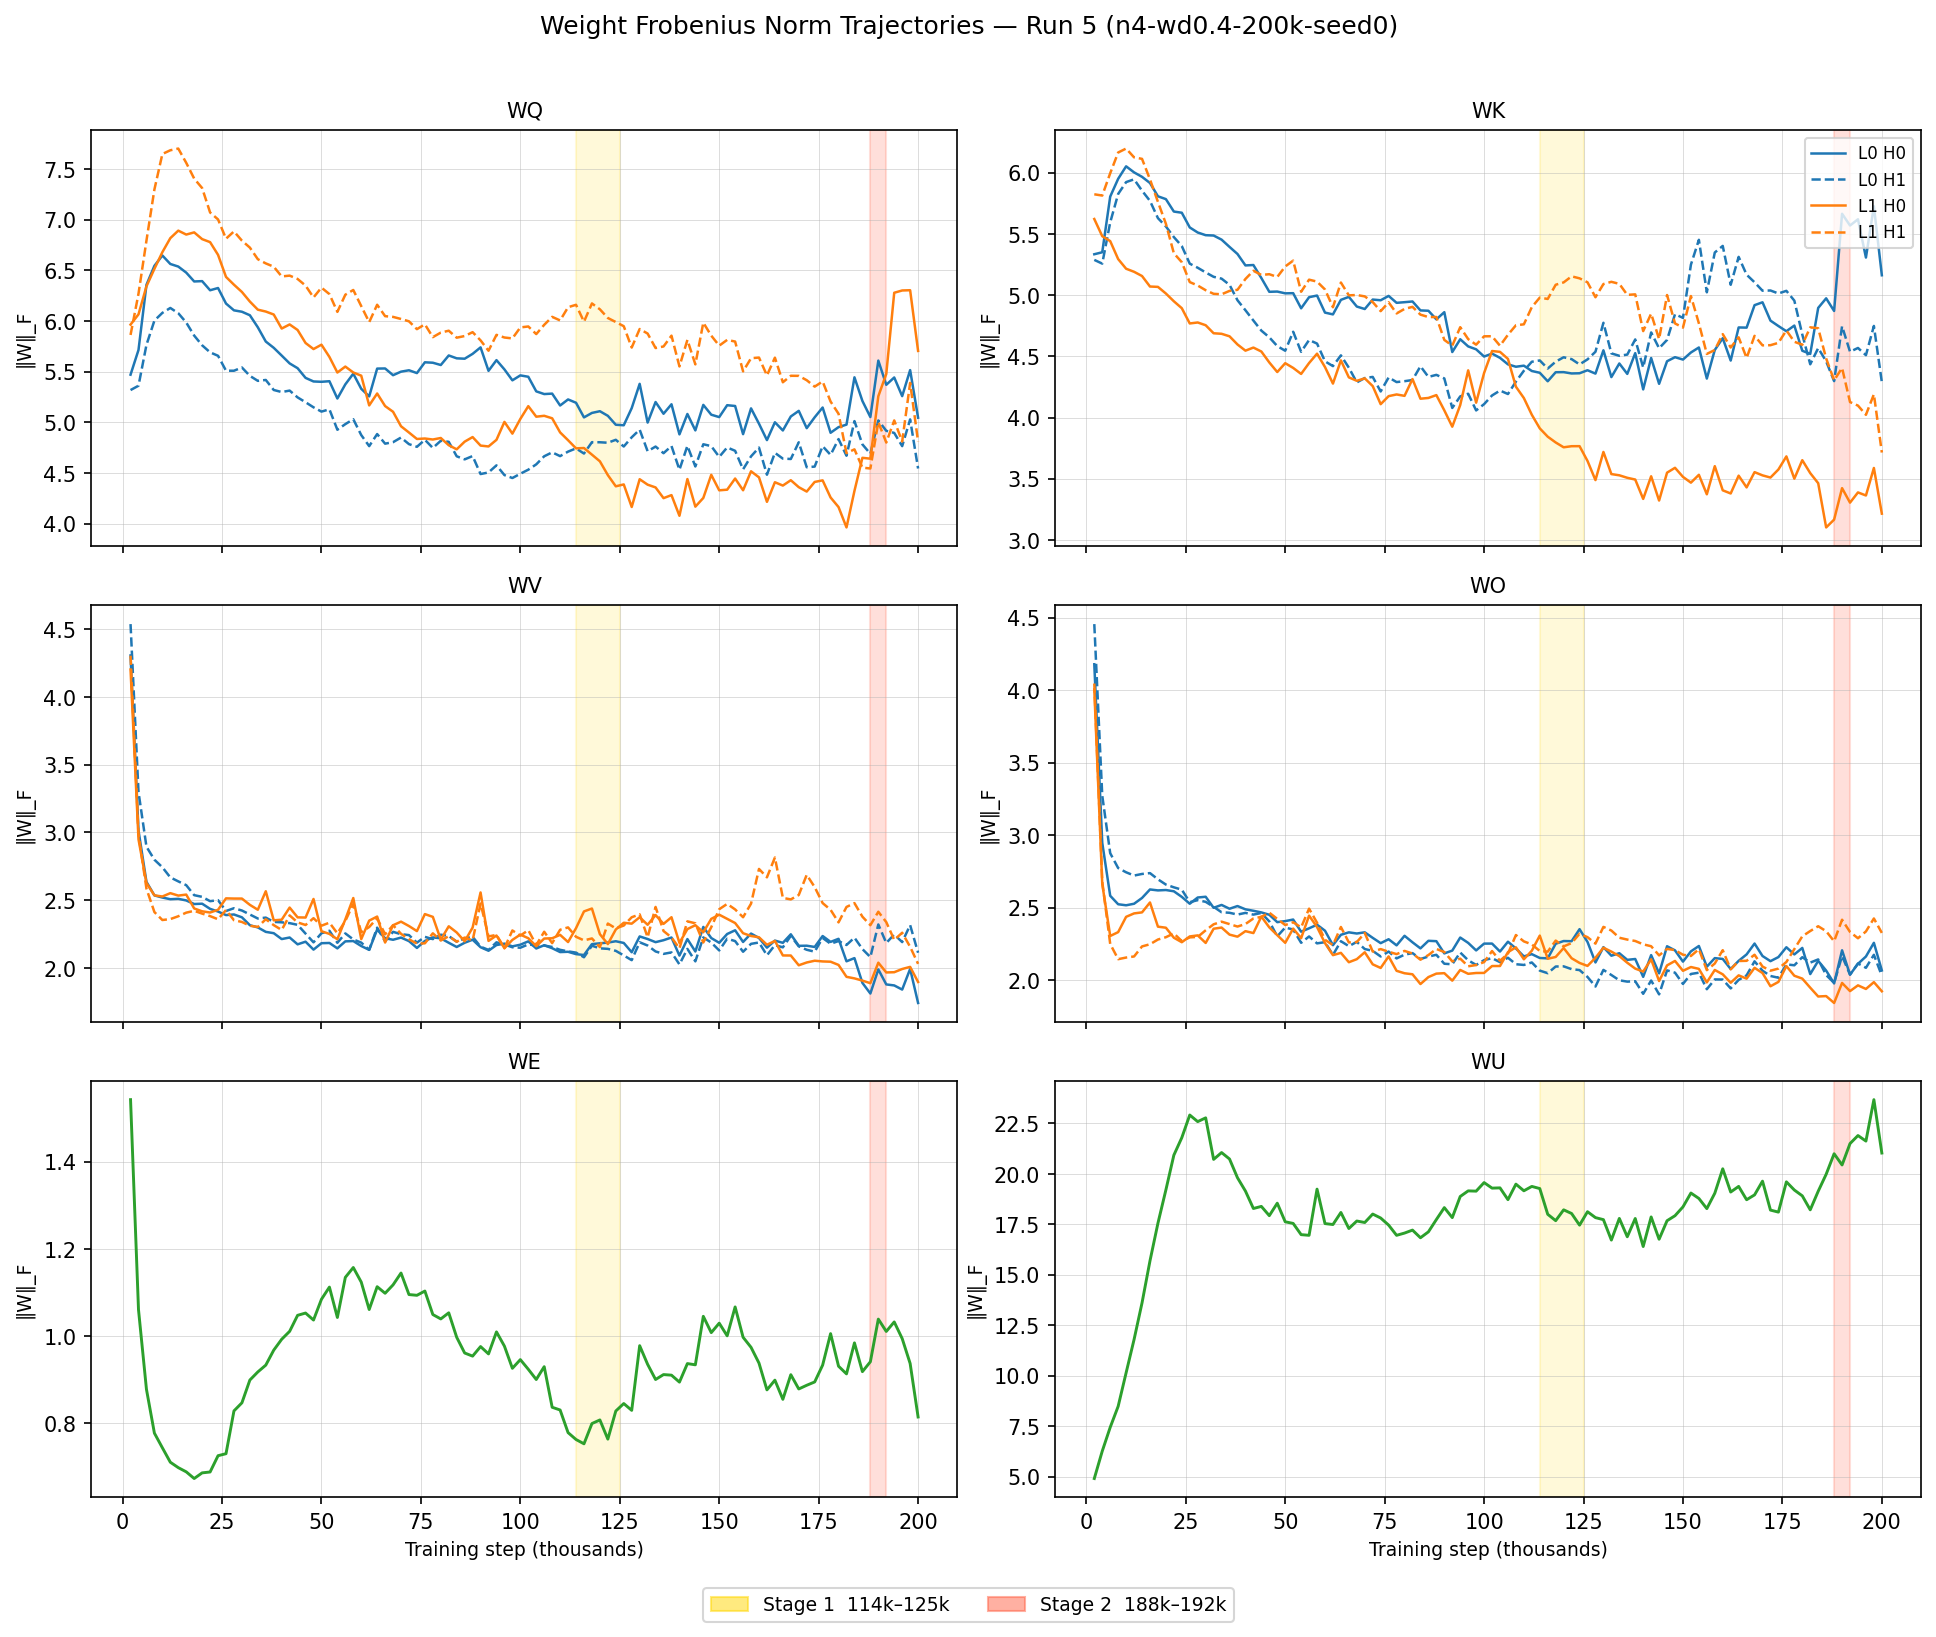
\includegraphics[width=\textwidth]{weight_norms.png}
\caption{Frobenius norm trajectories for all weight matrices over all
  100 checkpoints.  Color: blue = Layer~0, orange = Layer~1;
  line style: solid = Head~0, dashed = Head~1.  Orange shaded band:
  Stage~1 window (114k--125k).  Yellow shaded band: Stage~2 window
  (188k--192k).  L0H1's $W_V$ and $W_O$ norms grow sharply at
  Stage~2 ($+97\%$ from 126k to 196k), while Layer~1 norms are
  relatively flat across Stage~2.  Stage~1 is not visible in individual
  norms: the shortcut it builds is a matrix-alignment event, not a
  growth event.}
\label{fig:weight-norms}
\end{figure}

The weight-norm trajectories reveal the asymmetry between the two
stages.  Stage~2 is visible as a sharp rise in L0H1's $W_V$ and $W_O$
norms --- the matrices that form the OV circuit of the head that learns
the token-identity routing circuit (Section~\ref{sec:l0h1}).
Stage~1 produces no comparable individual-norm signature: no single
matrix suddenly grows large.  What changes at Stage~1 is the
\emph{alignment} between L1H0's and L1H1's $W_V W_O$ products and the
token embedding space --- a coordination event that is invisible to any
single norm.  This is why the OV circuit (the composed product
$W_E W_V W_O W_U$) is the correct unit of analysis.

% =============================================================================
\section{Circuit Analysis}
\label{sec:circuits}
% =============================================================================

Each attention head $h$ in layer $l$ performs two separable operations:

\begin{itemize}[noitemsep]
  \item \textbf{Routing} (QK circuit): which sequence positions does this
    head attend to?  Determined by
    $\mathrm{scale} \cdot W_E W_Q W_K^\top W_E^\top$, the
    token-type attention score matrix.  Entry $[i,j]$ is the score
    contribution when the query position holds token type $i$ and a
    key position holds type $j$.

  \item \textbf{Writing} (OV circuit): what information does it write
    to the residual stream when attending to a given token type?
    Determined by $W_E W_V W_O W_U$, the full token-to-logit
    projection.  Entry $[i,j]$ is the logit-$j$ contribution when this
    head attends to a position holding token type $i$.
\end{itemize}

Both circuits are computable directly from weights, without running
forward passes on specific inputs.  Analyses below compare two anchor
checkpoints: step~126k (immediately after Stage~1; the shortcut is
fully formed) and step~196k (after Stage~2; the final algorithm is in
place).

\subsection{Stage 1: the PAD-bias shortcut}
\label{sec:stage1}

\begin{figure}[H]
\centering
\begin{subfigure}[t]{0.48\textwidth}
  \centering
  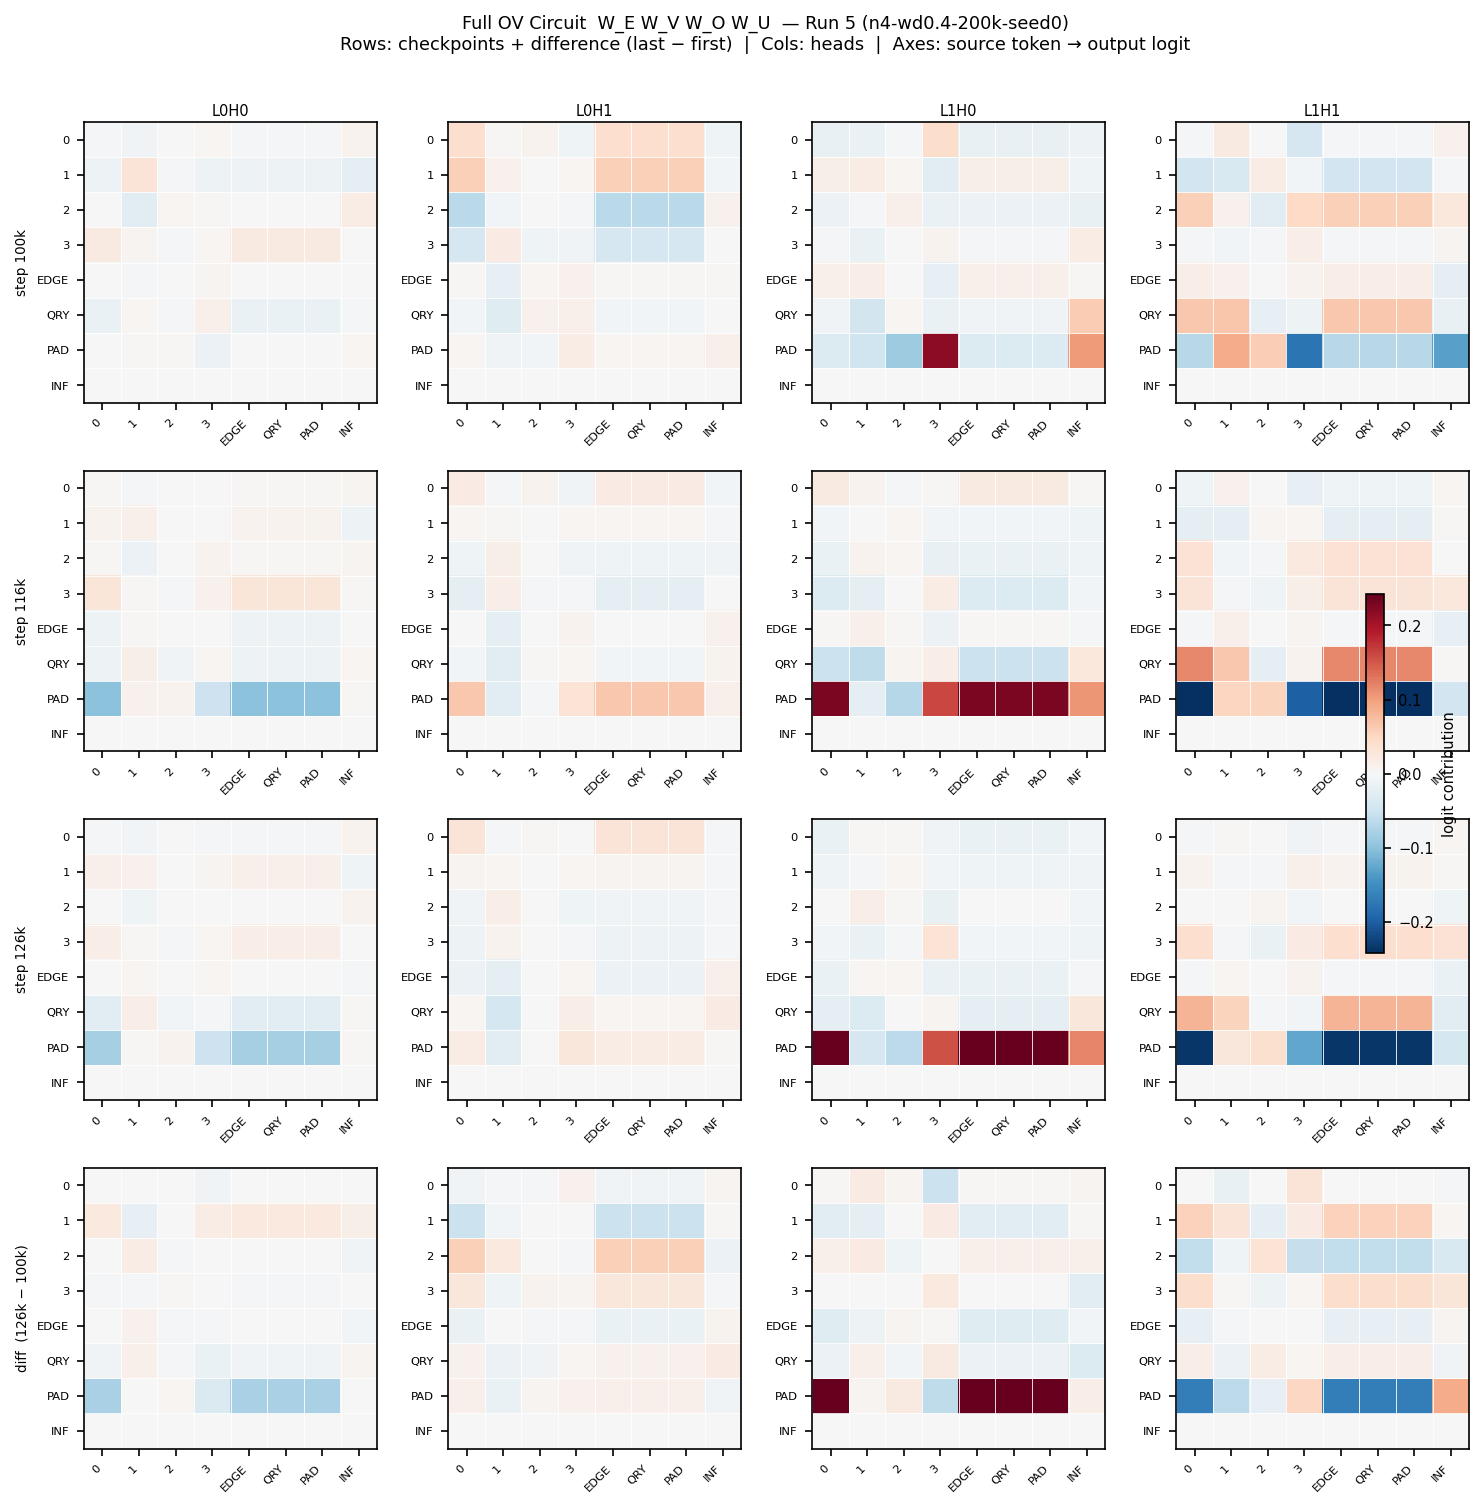
\includegraphics[width=\textwidth]{ov_circuits_stage1.png}
  \caption{OV circuits at Stage~1 (100k, 116k, 126k).}
  \label{fig:ov-stage1}
\end{subfigure}
\hfill
\begin{subfigure}[t]{0.48\textwidth}
  \centering
  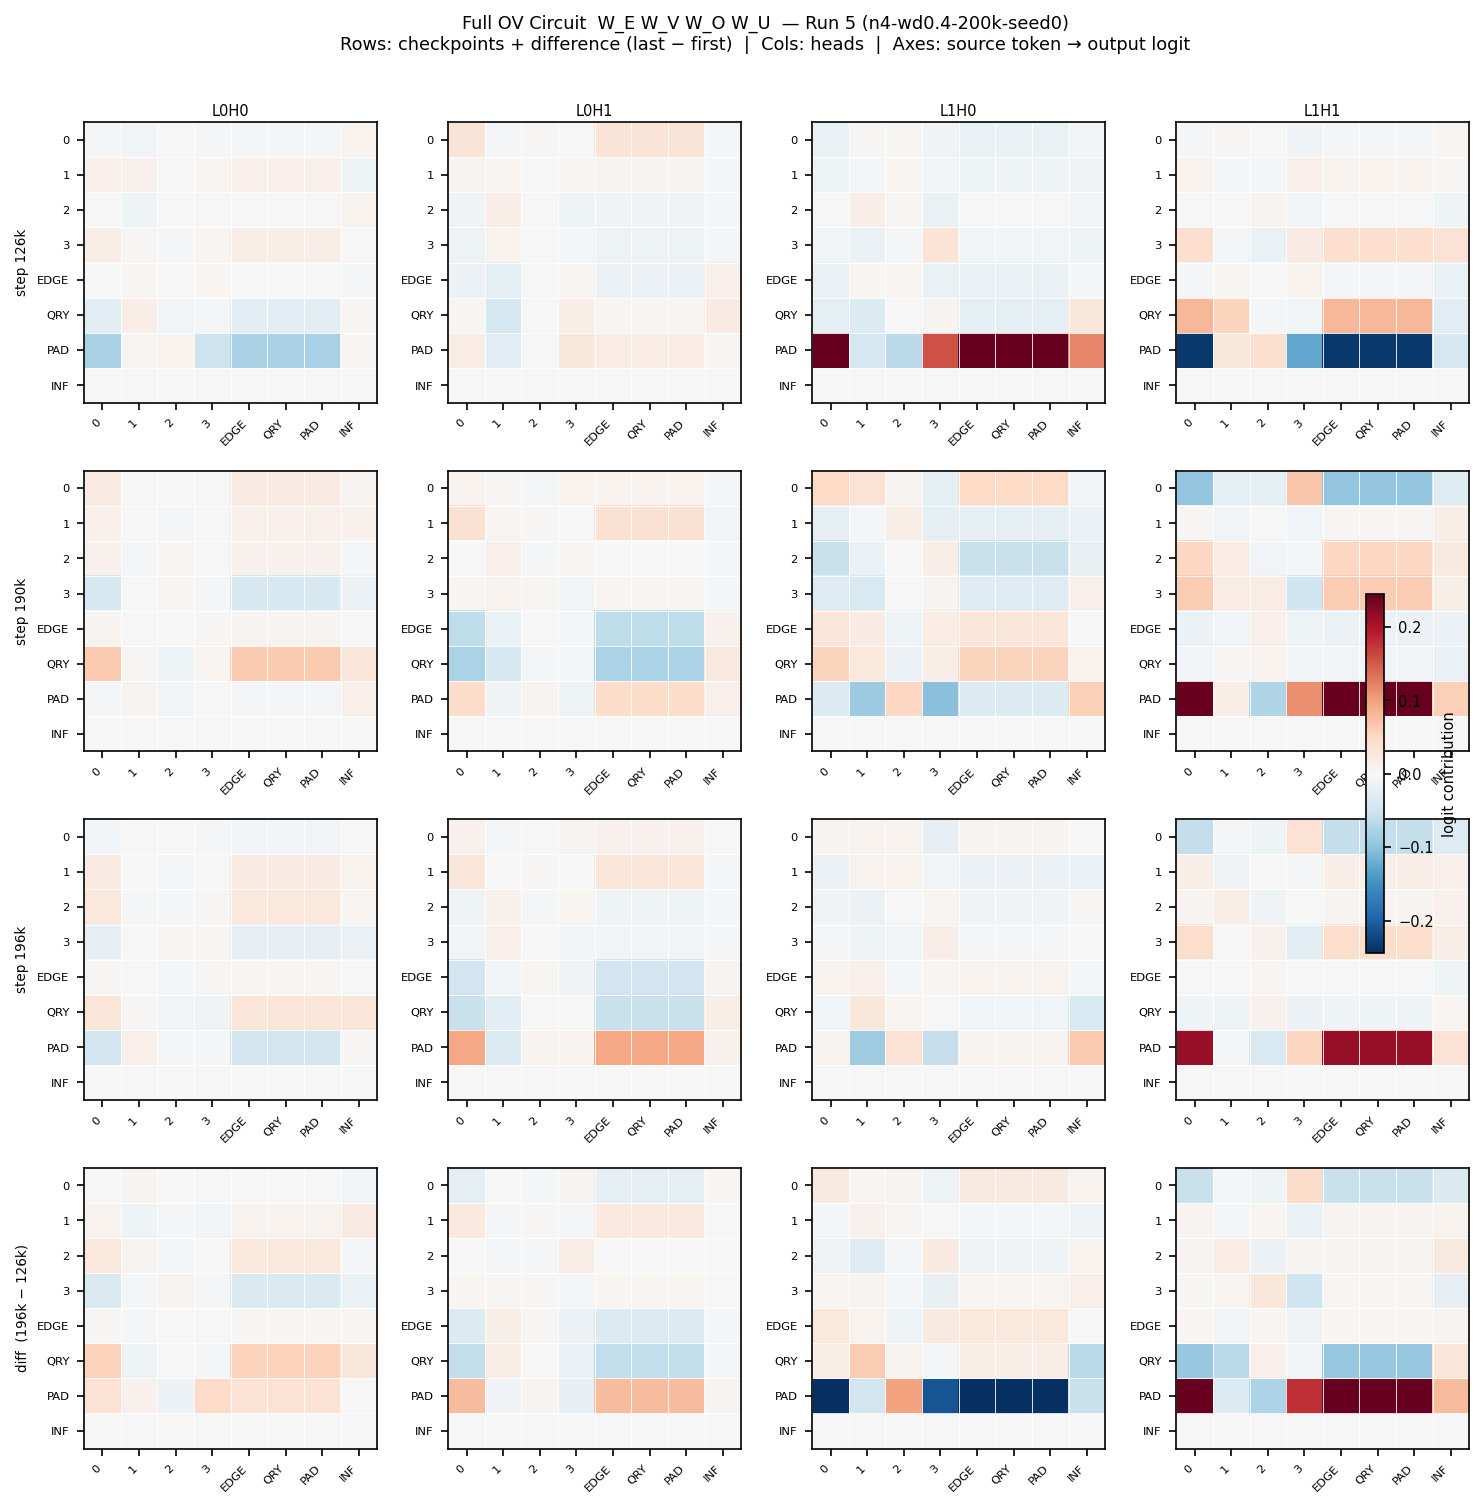
\includegraphics[width=\textwidth]{ov_circuits.png}
  \caption{OV circuits at Stage~2 (126k, 190k, 196k).}
  \label{fig:ov-stage2}
\end{subfigure}
\caption{Full OV circuit matrices $W_E W_V W_O W_U$ for all four heads
  at three checkpoints each, plus a difference row.  Rows = attended
  token type; columns = output logit.  RdBu\_r colormap; symmetric
  scale.  At Stage~1, the \PAD\ row (bottom) grows large in L1H0 and
  L1H1, indicating those heads develop a structured PAD-position
  projection.  At Stage~2, L0H1's matrix grows substantially while
  L1's PAD-row structure weakens and partially reverses.}
\label{fig:ov-circuits}
\end{figure}

By step~126k, Layer~1 heads (L1H0 and L1H1) have developed a striking
pattern in their OV circuits: the \PAD\ token row is the largest in
the matrix.  When these heads attend to a padding position, they
inject a non-trivial logit bias: L1H0 pushes valid-answer logits
toward longer distances and $\INF$, while impossible-answer tokens
(node~0, \EDGE, \QRY, \PAD) are grouped at a common maximum.

This is the PAD-bias shortcut.  Sequences for 4-node graphs contain
approximately 21\% padding positions.  By Step~126k, L1H0 has also
developed near-uniform attention weights, so the PAD contribution
is always active: roughly 21\% of its attention mass lands on \PAD\
tokens in every forward pass, always adding the same logit offset.
The model has learned to inject a constant ``prefer unreachability and
long distances'' prior --- statistically useful on sparse directed
graphs, but not a computation of the actual answer.

\paragraph{Causal validation.}
To confirm the shortcut is load-bearing, we ablate PAD-position
attention weights in Layer~1 across four checkpoints and measure the
accuracy drop:

\begin{table}[H]
\centering
\begin{tabular}{@{}lcc@{}}
\toprule
Checkpoint & Drop (no renorm) & Drop (renorm) \\
\midrule
100k (pre-Stage~1) & $-0.6\%$ & $-1.2\%$ \\
126k (post-Stage~1) & $\mathbf{-2.9\%}$ & $\mathbf{-4.1\%}$ \\
160k (plateau)      & $-2.4\%$ & $-3.5\%$ \\
196k (post-Stage~2) & $-1.3\%$ & $-2.0\%$ \\
\bottomrule
\end{tabular}
\caption{Accuracy drop when PAD-position attention weights in Layer~1
  are zeroed.  Largest effect at 126k, confirming the shortcut is most
  load-bearing at Stage~1.  Stage~2 substantially reduces dependence
  but does not fully eliminate it.  The renormalized variant
  consistently hurts more, indicating PAD key positions carry a
  specific beneficial value signal that is distinct from their attention
  weight magnitude.}
\label{tab:ablation}
\end{table}

The ablation effect peaks at 126k ($-2.9\%$) and declines at 196k
($-1.3\%$), tracing exactly the arc predicted by the mechanistic
account: the shortcut is built at Stage~1 and partially dismantled at
Stage~2.

\subsection{Stage 2: L0H1 grows and routes}
\label{sec:stage2}

The dominant structural change at Stage~2 is the growth of L0H1.  Its
OV circuit norm increases by $+97\%$ from step~126k to step~196k ---
the largest single-head change across the entire training run.
Simultaneously, its QK circuit crystallizes into a clean token-identity
matching pattern.

\subsubsection{L0H1 QK circuit: ``find edges involving dst''}
\label{sec:l0h1}

\begin{figure}[H]
\centering
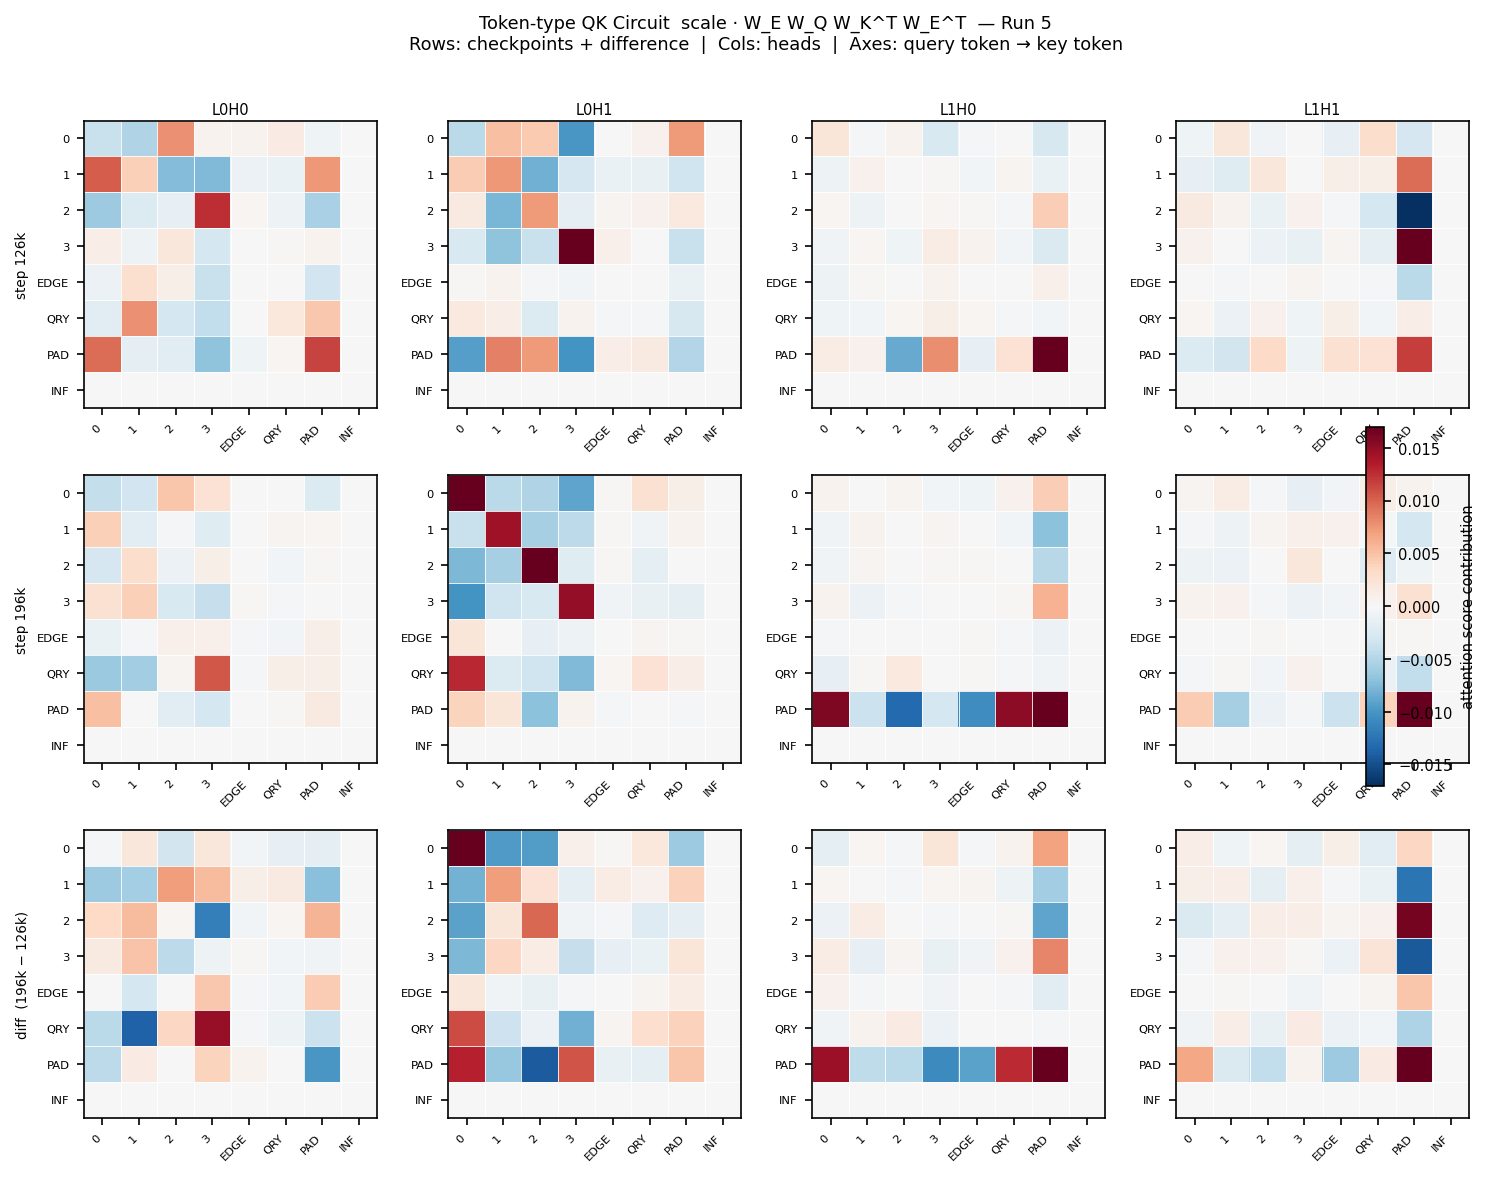
\includegraphics[width=\textwidth]{qk_circuits.png}
\caption{L0H1 at step~196k shows a diagonal-dominant pattern over the
  node-token subblock, indicating that destination tokens preferentially
  attend to positions holding the same node token --- implementing
  ``find edges involving dst.''  This crystallization is absent at
  step~126k and emerges during Stage~2 simultaneously with L0H1's OV
  norm growth.  The other three heads show no comparable structured
  routing: L0H0 entries are small and inconsistent across checkpoints;
  L1H0 and L1H1 instead show PAD self-attraction (QK[\PAD, \PAD] is the
  matrix maximum at both checkpoints), reinforcing their role in the
  bias shortcut.  Rows = query token type; columns = key token type;
  RdBu\_r colormap, symmetric scale.}
\label{fig:qk-circuits}
\end{figure}

At step~196k, L0H1's node-token subblock of the QK matrix is
strongly diagonal-dominant:

\begin{center}
\begin{tabular}{lrrrr}
\toprule
query $\backslash$ key & node~0 & node~1 & node~2 & node~3 \\
\midrule
node~0 & $\mathbf{+0.018}$ & $-0.005$ & $-0.005$ & $-0.009$ \\
node~1 & $-0.004$ & $\mathbf{+0.014}$ & $-0.006$ & $-0.004$ \\
node~2 & $-0.008$ & $-0.006$ & $\mathbf{+0.017}$ & $-0.002$ \\
node~3 & $-0.010$ & $-0.003$ & $-0.003$ & $\mathbf{+0.015}$ \\
\bottomrule
\end{tabular}
\end{center}

Each node token type preferentially attends to sequence positions
holding the \emph{same} node token.  Because the prediction is read
from the \texttt{dst} position (which holds the destination node token
as its embedding), L0H1 attends toward all positions in the sequence
that also contain the destination token --- precisely the edge triplets
in which the destination node appears as either source or destination.

This is the first step of a backward reachability search: \textbf{L0H1
implements ``find edges involving the destination node.''} At
step~126k, the diagonal is present but noisy; by step~196k it is
clean and consistent across all four node values.  Both the routing
(QK) and writing (OV) components of L0H1 develop simultaneously during
Stage~2.

\subsubsection{L0H1 OV circuit: what it writes}

\begin{figure}[H]
\centering
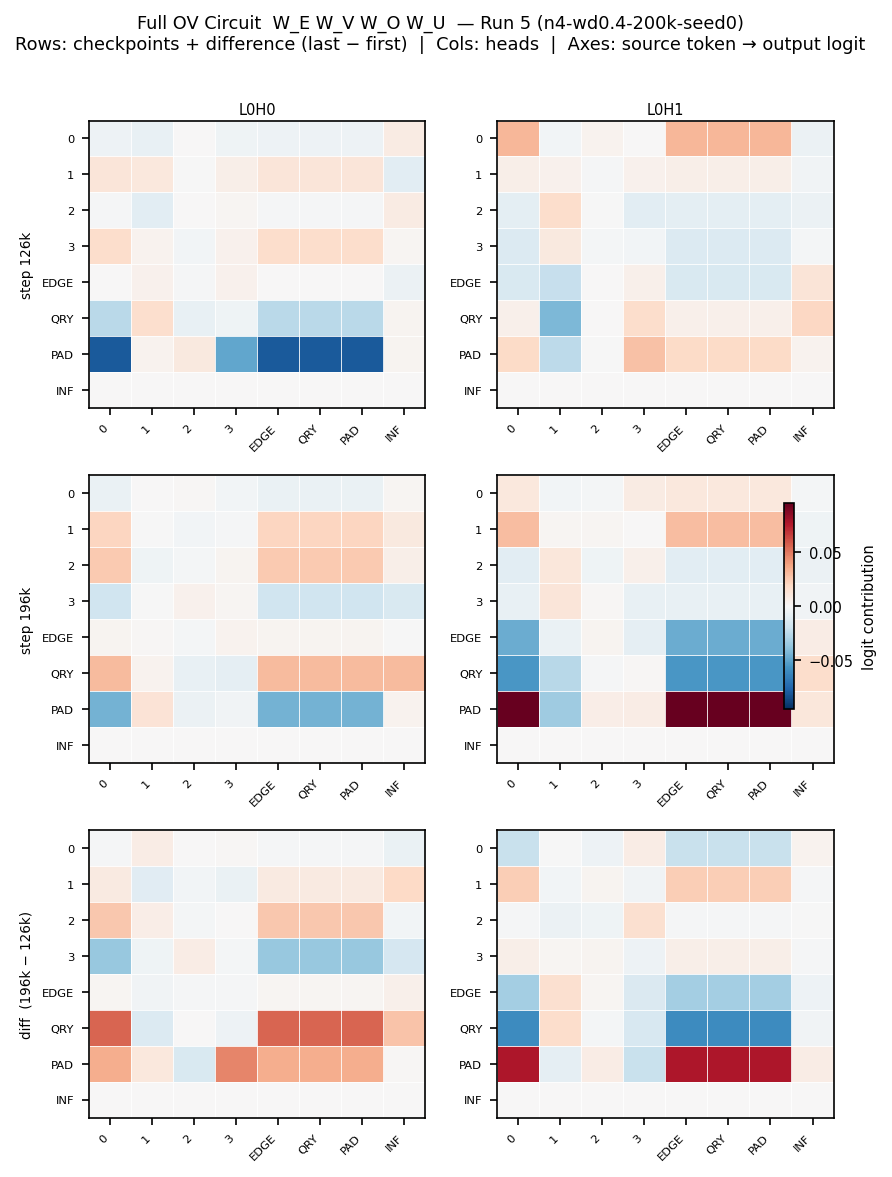
\includegraphics[width=\textwidth]{ov_l0_circuits.png}
\caption{L0H1 OV circuit ($W_E W_V W_O W_U$) at steps 126k and 196k
  for Layer~0 heads.  L0H1 grows substantially from 126k to 196k.
  The node-token rows (0--3) show a node-conditioned pattern; the
  impossible-answer tokens cluster at identical values within each row.
  L0H0 shows no comparable structured growth.}
\label{fig:ov-l0}
\end{figure}

When L0H1 attends to a position holding node token $i$, it writes a
node-conditioned logit offset to the residual stream:

\begin{table}[H]
\centering
\caption{L0H1 OV circuit: node-token rows at step~196k.  Each entry is
  the logit contribution when L0H1 attends to that token type.
  Impossible-answer tokens (node~0 excluded; \EDGE, \QRY, \PAD) are
  grouped at identical values in every row, marked $c$.}
\label{tab:l0h1-ov}
\begin{tabular}{@{}lrrrrr@{}}
\toprule
Attended token & dist=1 & dist=2 & dist=3 & \INF & $c$ \\
\midrule
node~0 & $-0.003$ & $-0.002$ & $\mathbf{+0.008}$ & $-0.002$ & $+0.010$ \\
node~1 & $+0.002$ & $+0.002$ & $+0.000$ & $-0.004$ & $+0.029$ \\
node~2 & $\mathbf{+0.011}$ & $-0.004$ & $+0.005$ & $-0.006$ & $-0.010$ \\
node~3 & $\mathbf{+0.012}$ & $+0.001$ & $-0.007$ & $-0.003$ & $-0.007$ \\
\bottomrule
\end{tabular}
\end{table}

Nodes~2 and~3 push the dist=1 logit most strongly ($+0.011$ and
$+0.012$); node~0 pushes toward dist=3 ($+0.008$); node~1 is nearly
neutral.

Three caveats are important.  First, the effect sizes are modest
(0.008--0.012 logit units).  Second, the formula $W_E W_V W_O W_U$
captures the token-type component of the value vectors only; the full
value at an attended position also contains a positional term
$W_V W_{\mathrm{pos}}[p]$ that depends on where in the sequence the
position sits.  Given that node-token ranges (0.013--0.034) are small
relative to the \PAD\ row (0.129), the positional component almost
certainly carries the dominant structural signal --- specifically, the
discrimination between positions where the destination node appears as
an edge \emph{destination} (predecessors of dst, directly useful for
path-finding) versus an edge \emph{source} (successors of dst, less
directly useful).  Third, the node-conditioned prior plausibly reflects
statistical regularities in the training distribution rather than a
structural computation, though we have not directly verified this.
The prior is real and measurable; how much of Layer~0's accuracy it
explains versus the positional component remains open.

\subsubsection{L1H0 and L1H1: PAD self-routing}

Layer~1 heads route attention toward \PAD\ positions not only through
the magnitude structure of the key vectors but also through a learned
token-type affinity.  L1H0's QK[PAD, PAD] grows from $+0.029$ at
step~126k to $+0.058$ at step~196k --- the largest single entry in any
head's QK matrix.  L1H1's QK[PAD, PAD] is $+0.044$ at step~196k.
This PAD self-attraction reinforces the OV analysis: Layer~1 heads are
structured to attend to \PAD\ positions, which is the routing
mechanism behind the bias shortcut.

% =============================================================================
\section{The Learned Algorithm}
\label{sec:algorithm}
% =============================================================================

\subsection{Logit lens decomposition}

The logit lens \citep{nostalgebraist2020} projects the residual stream
at each layer through $\LN_{\mathrm{final}}$ and $W_U$ to read the
model's partial prediction at intermediate depths.  For this 2-layer
model, there are three depths: the raw embeddings only (before any
attention), after Layer~0, and after Layer~1 (the full model).

\begin{table}[H]
\centering
\caption{Logit lens accuracy by depth and answer category.  Steps 126k
  and 196k.  $n$ = validation examples per category (total: 480).
  $\Delta$ L1 = full model minus after-L0.}
\label{tab:logit-lens}
\begin{tabular}{@{}llrrrrrr@{}}
\toprule
Step & Depth & Overall &
  dist=1 ($n$=181) & dist=2 ($n$=92) &
  dist=3 ($n$=21) & \INF\ ($n$=186) \\
\midrule
126k & embed only  & 37.7\% & 100.0\% & 0.0\%  & 0.0\%  & 0.0\%  \\
     & after L0    & 45.6\% & 79.6\%  & 10.9\% & 4.8\%  & 34.4\% \\
     & full model  & 81.0\% & 90.1\%  & 55.4\% & 19.0\% & 91.9\% \\
     & $\Delta$ L1 &        & $+10.5\pp$ & $+44.6\pp$ & $+14.3\pp$ & $+57.5\pp$ \\
\midrule
196k & embed only  & 34.6\% & 75.7\%  & 31.5\% & 0.0\%  & 0.0\%  \\
     & after L0    & 57.5\% & 77.9\%  & 17.4\% & 47.6\% & 58.6\% \\
     & full model  & 92.5\% & 99.4\%  & 87.0\% & 23.8\% & 96.2\% \\
     & $\Delta$ L1 &        & $+21.5\pp$ & $\mathbf{+69.6\pp}$ &
       $\mathbf{-23.8\pp}$ & $+37.6\pp$ \\
\bottomrule
\end{tabular}
\end{table}

The table tells a precise algorithmic story.

\paragraph{Layer 0 handles distance-1.}
After Layer~0 at step~196k, 77.9\% of distance-1 queries are already
answered correctly --- only 21.5 percentage points below the full
model's 99.4\%.  This is exactly what the QK circuit predicts: L0H1's
token-identity matching routes the dst-position query toward all edge
triplets containing the destination token, and the OV contribution is
sufficient to answer most direct adjacency queries correctly.  Layer~0
is the primary circuit for distance-1.

\paragraph{Layer 1's dominant contribution is distance-2 ($+69.6\pp$).}
Layer~0 alone achieves only 17.4\% on distance-2 examples; the full
model achieves 87.0\%.  Layer~1 provides essentially all of the 2-hop
reasoning.  This is consistent with a two-step backward BFS: Layer~0
collects predecessors of dst; Layer~1 checks whether src can reach any
of those predecessors in one hop --- identifying a path
$\mathrm{src} \to x \to \mathrm{dst}$.

\paragraph{Layer 1 hurts distance-3 ($-23.8\pp$).}
After Layer~0 at step~196k, 47.6\% of distance-3 queries are correct
(10 of 21 examples).  After Layer~1, this falls to 23.8\% (5 of 21).
Layer~1 actively misclassifies 3-hop paths.  The mechanism is
straightforward: for a path $\mathrm{src} \to x \to y \to \mathrm{dst}$,
Layer~0 identifies $y$ as a direct predecessor of dst; Layer~1 then
checks whether src can reach $y$ in one hop --- it cannot (src reaches
$y$ only through $x$) --- and concludes that no predecessor of dst is
reachable, routing the prediction toward $\INF$ or a shorter distance.
This is not a training failure; it is an architectural constraint.  A
two-layer backward BFS cannot resolve a three-edge path.

\paragraph{Layer 1's INF contribution at Stage 1 was the shortcut.}
At step~126k, Layer~1's largest contribution is $+57.5\pp$ on $\INF$
cases.  This is the PAD-bias shortcut in action: by injecting a
constant logit offset toward $\INF$ and longer distances through PAD
attention, Layer~1 raises $\INF$ accuracy from 34.4\% (after L0) to
91.9\% (full model).  By step~196k, that same contribution is provided
by the genuine path-checking circuit rather than the shortcut --- the
$\INF$ contribution is now $+37.6\pp$, but it comes from structurally
reasoning about reachability rather than from a statistical bias.

\subsection{The algorithm: a complete narrative}

The fully trained model (step~196k) processes a shortest-path query as
follows.

\paragraph{Input.}
The model receives 21 tokens encoding a 4-node directed graph and a
query.  Each directed edge $a \to b$ is encoded as
$[\EDGE,\, a,\, b]$; unused edge slots are filled with $\PAD$.  The
final three tokens are $[\QRY,\, \mathrm{src},\, \mathrm{dst}]$.  The
prediction is read from the \texttt{dst} position.

\paragraph{Layer 0: collecting dst's neighborhood.}
L0H1's token-identity QK circuit routes the dst-position query toward
every sequence position that holds the same node token as dst.  In the
edge list, these are the triplets in which the destination node appears
as either an edge source or an edge destination --- the immediate
neighborhood of dst.  L0H1 writes this neighborhood information back
to the residual stream as an OV contribution with two components: a
node-conditioned distance prior (modest in magnitude, likely reflecting
training distribution statistics) and a positional component that
distinguishes edge positions by their structural role.  Together, these
allow Layer~0 to answer $\approx$78\% of distance-1 queries correctly.
L0H0 contributes a weaker, less structured signal.

\paragraph{Layer 1: completing the path check.}
Layer~1 reads the residual stream at the dst position, which now
encodes dst's neighborhood from Layer~0.  It performs the critical
second step: checking whether src can reach any of dst's direct
predecessors.

\begin{itemize}[noitemsep]
  \item \textbf{Distance-1} (src $\to$ dst directly): src is itself a
    direct predecessor of dst.  Layer~1 confirms the connection
    ($+21.5\pp$ over Layer~0's already strong 77.9\% baseline).

  \item \textbf{Distance-2} (src $\to x \to$ dst): $x$ is a direct
    predecessor of dst, identified by Layer~0; Layer~1 confirms that
    src has a direct edge to $x$.  This is Layer~1's primary
    contribution ($+69.6\pp$).

  \item \textbf{INF} (dst unreachable from src): no predecessor of dst
    is reachable from src in one hop.  Layer~1 confirms the absence of
    a connecting edge ($+37.6\pp$).
\end{itemize}

\paragraph{Caveat on Layer~1's mechanism.}
The logit lens establishes that Layer~1 is causally responsible for the
$+69.6\pp$ improvement on distance-2, and the backward BFS account is
the most parsimonious explanation consistent with all circuit analyses
in this work.  However, we have not traced this computation directly
through Layer~1's QK or OV circuits at step~196k --- we have not
identified which head is responsible, which token positions it attends
to, or how it reads the predecessor information written by Layer~0.
The two-step backward BFS description is the best-supported hypothesis,
not a fully characterized circuit.  Completing this trace is the
clearest direction for future work.

\paragraph{Distance-3 and the architectural limit.}
For a 3-hop path $\mathrm{src} \to x \to y \to \mathrm{dst}$, Layer~0
identifies $y$ as a direct predecessor of dst.  Layer~1 checks whether
src can directly reach $y$ --- it cannot.  Layer~1 therefore concludes
that no predecessor of dst is directly reachable from src, and pushes
the prediction toward $\INF$ or a shorter distance.  The model achieves
only 23.8\% on distance-3 examples, compared to 47.6\% from Layer~0
alone.  A two-layer backward BFS cannot handle a three-edge path; this
is an architectural limitation, not a training failure.

\paragraph{Summary.}
This model implements a \textbf{partial two-step backward BFS from the
destination node}, one BFS step per layer.  Layer~0 collects the set of
nodes adjacent to dst; Layer~1 checks whether src can reach any of
those nodes directly.  Distances 1 and 2 are handled well; distance 3
exceeds the architecture's depth.  The two accuracy jumps in the
training curve are not two instances of the same phenomenon: Stage~1
is the \emph{construction} of a statistical shortcut (PAD-position
logit bias), and Stage~2 is its \emph{replacement} by a genuine
graph-structural computation.

% =============================================================================
\section{Discussion}
\label{sec:discussion}
% =============================================================================

\subsection{Why two stages?}

The double-grokking pattern under $\lambda = 0.4$ reflects the model
assembling its algorithm in two components that cross their respective
generalization thresholds at different times.  At $\lambda = 0.2$, the
same two components develop but their transitions overlap and appear as
a single sharp event.  The slower compression under $\lambda = 0.4$
separates their timescales, making the mechanistic structure visible.

The Stage~1 shortcut --- attending to padding positions to inject a
constant logit bias --- is a genuine local minimum in the optimization
landscape.  The constant bias is statistically useful (sparse directed
graphs have many unreachable pairs), and it requires less structural
complexity than learning to route attention by token identity.  Stage~1
is not a failed attempt at the correct solution; it is the best
solution the model can find under the weight constraints of the
Stage~1 plateau.  Stage~2 only becomes possible after continued weight
decay has compressed the shortcut enough that the gradient can carve
out a lower-loss path toward the structural circuit.

\subsection{What the architecture can and cannot do}

The two-layer design places a hard ceiling at 2-hop paths.  Each
attention layer implements one step of backward BFS from the
destination.  Distance-3 paths require three steps; with only two
layers, the model cannot perform the third step, and Layer~1's
computation actively interferes with Layer~0's partial answer.
The $-23.8\pp$ Layer~1 degradation on distance-3 is not noise; it is a
systematic misclassification that follows directly from the mismatch
between the algorithm the model has learned and the task structure it
cannot handle.

A 3-layer model should be able to handle distance-3.  Testing this
prediction --- and checking whether the same staged grokking pattern
appears, now with three stages --- is the most direct extension of this
work.

\subsection{Implications for grokking research}

Prior grokking analyses focused on the single transition from
memorization to generalization.  This work shows that the transition
can split into multiple mechanistically distinct events when weight
decay is strong enough to separate their timescales.  The first event
is not just a ``partial'' version of the second: Stage~1 (shortcut
construction) and Stage~2 (shortcut replacement) are qualitatively
different in the type of computation they establish.

This has implications for how grokking should be studied.  Analyzing
only the final checkpoint misses the intermediate shortcut phase and
the Stage~1 to Stage~2 transition, which is where the most interesting
computation reorganization occurs.  Dense checkpoint logging across the
full training run --- not just before and after --- is necessary to
catch this structure.

Concretely: a study that examined only the converged model in this work
would have found a partial backward BFS circuit and reported that as the
learned algorithm.  It would have missed entirely that this circuit was
preceded by a qualitatively different solution --- a PAD-bias shortcut
--- which was the model's ``learned algorithm'' for thousands of
training steps.  The shortcut is not a transient artifact; it is stable
for 63{,}000 steps across a plateau and causes the model to achieve
above-80\% accuracy without performing any graph computation.  We
suspect this pattern --- an intermediate statistical shortcut that is
stable, above chance, and mechanistically distinct from the final
solution --- may be common in tasks where a cheap structural regularity
in the input is available to exploit before the true algorithmic
solution becomes accessible.  If so, the field's current practice of
studying only converged models systematically underestimates the
complexity of how algorithmic generalization is acquired.

\subsection{Limitations and future work}

\paragraph{The positional OV component is uncharacterized.}
The token-type OV analysis captures only part of L0H1's value
contribution.  The positional term $W_V W_{\mathrm{pos}}[p]$, which
varies with where in the sequence an attended position sits, is
excluded from the $W_E W_V W_O W_U$ decomposition.  Given that
token-type ranges (0.013--0.034) are small relative to the \PAD\ row
(0.129), this positional component almost certainly carries the
dominant structural signal --- discriminating between positions where
dst appears as an edge destination (predecessors of dst) versus an
edge source (successors of dst).  Characterizing this positional
component requires a position-level analysis not performed here.

\paragraph{Layer~1's circuit at Step~196k is not directly traced.}
The logit lens establishes Layer~1's causal role in 2-hop reasoning.
The circuit-level mechanism --- which head is responsible, which token
positions it attends to, how it reads Layer~0's output --- remains
uncharacterized.  Completing this trace would give a fully mechanistic
account of the backward BFS.

\paragraph{Scope: 4-node graphs only.}
All experiments use 4-node graphs, producing a dataset of 1{,}920
training examples.  Whether the same circuit appears on larger graphs
(6, 8, 10 nodes), whether grokking still occurs, and whether the
two-stage pattern persists are open questions.  The task difficulty
scales with $n$: longer sequences, more edge triplets, deeper BFS
required for longer paths.

% =============================================================================
\begin{thebibliography}{9}

\bibitem[Cohen et~al.(2025)]{cohen2025spectral}
A.~Cohen, A.~Gromov, K.~Yang, and Y.~Tian.
\newblock Spectral journey: How transformers predict the shortest path.
\newblock \emph{arXiv preprint arXiv:2502.08794}, 2025.

\bibitem[Elhage et~al.(2021)]{elhage2021mathematical}
N.~Elhage, N.~Nanda, C.~Olsson, T.~Henighan, N.~Joseph, B.~Mann,
A.~Askell, Y.~Bai, A.~Chen, T.~Conerly, et~al.
\newblock A mathematical framework for transformer circuits.
\newblock \emph{Transformer Circuits Thread}, 2021.
\newblock \url{https://transformer-circuits.pub/2021/framework/index.html}

\bibitem[nostalgebraist(2020)]{nostalgebraist2020}
nostalgebraist.
\newblock Interpreting GPT: the logit lens.
\newblock \emph{LessWrong}, 2020.
\newblock \url{https://www.lesswrong.com/posts/AcKRB8wDpdaN6v6ru/interpreting-gpt-the-logit-lens}

\bibitem[Power et~al.(2022)]{power2022grokking}
A.~Power, Y.~Burda, H.~Edwards, I.~Babuschkin, and V.~Misra.
\newblock Grokking: generalization beyond overfitting on small algorithmic
  datasets.
\newblock \emph{arXiv:2201.02177}, 2022.

\end{thebibliography}

\end{document}
